%%%%%%%%%%%%%%%%%%%%%%%%%%%%%%%%%%%%%%%%%%%%%%%%%%%%%%%%%%%%%%%%%%%%%%%%%%%%%
%% 03_arch_bus_concept.tex
%% Section: Bus Concept
%% Chapter: Architecture Concepts
%%
%% Describes the dual-bus architecture of the RWU-RV64I chip:
%%   - Wishbone B4 Classic for CPU-to-peripheral access
%%   - AMBA AXI4 (read-only subset) for cache-to-memory-arbiter path
%%
%% Integration in 00_rwurv64i_all.tex:
%%   \section{Bus Concept}
%%   \input{\TEXTarch 03_arch_bus_concept}
%%
%% Requires packages: tabularx, booktabs, tikz, float, xcolor, hyperref
%%
%% v0.1  2026-02-19  Claude-AI  Initial version (Wishbone only)
%% v0.2  2026-05-12  Claude-AI  Add AXI4 cache bus; dual-bus architecture
%%%%%%%%%%%%%%%%%%%%%%%%%%%%%%%%%%%%%%%%%%%%%%%%%%%%%%%%%%%%%%%%%%%%%%%%%%%%%

%%%%%%%%%%%%%%%%%%%%%%%%%%%%%%%%%%%%%%%%%%%%%%%%%%%%%%%%%%%%%%%%%%%%%%%%%%%%%
\subsection{Overview}
%%%%%%%%%%%%%%%%%%%%%%%%%%%%%%%%%%%%%%%%%%%%%%%%%%%%%%%%%%%%%%%%%%%%%%%%%%%%%

The RWU-RV64I chip uses a \textbf{dual-bus architecture} with two
independent on-chip buses serving different purposes:

\begin{itemize}
  \item \textbf{Wishbone B4 Classic} -- the peripheral bus.
    All configuration registers, GPIO, UART, and QSPI control registers
    are connected to the CPU via this bus.
    It was chosen for its simplicity, open-source IP availability, and
    compatibility with the existing peripheral IP blocks.

  \item \textbf{AMBA AXI4} (read-only subset) -- the cache memory bus.
    The I-Cache and D-Cache controllers use this bus to fetch 32-byte
    cache lines from NOR Flash via the Memory Arbiter and the QSPI
    controller data port.
    AXI4 was chosen for its burst capability: a 4-beat INCR burst fills
    one cache line in a single transaction instead of eight independent
    Wishbone single-cycle transfers.
\end{itemize}

The two buses are completely independent.
There is no bridge between them.
The Wishbone bus carries only single-word register accesses;
the AXI4 bus carries only 32-byte cache-line bursts.
Table~\ref{tab:asDualBus} summarises the key parameters of each bus.

\begin{table}[H]
\caption{On-Chip Bus Summary}
\label{tab:asDualBus}
\centering
\begin{tabularx}{\textwidth}{|l |l |l |X|}
  \hline
  Property          & Wishbone B4 Classic         & AXI4 (cache subset)      & Comment \\
  \hline
  \hline
  Purpose           & Peripheral access           & Cache line fill          & \\
  \hline
  Standard          & Wishbone B4 Classic         & AMBA AXI4                & \\
  \hline
  Data width        & 64\,bit                     & 64\,bit                  & \\
  \hline
  Address width     & 64\,bit                     & 32\,bit                  & Physical address only \\
  \hline
  Transfer type     & Single-word                 & 4-beat INCR burst        & ARLEN=3, ARSIZE=3 \\
  \hline
  Burst support     & No                          & Yes (read only)          & Write channels eliminated \\
  \hline
  Masters           & CPU core                    & I-Cache, D-Cache         & \\
  \hline
  Slaves            & GPIO, UART, QSPI cfg regs   & QSPI controller (data)   & \\
  \hline
  Arbitration       & Single master (no arbiter)  & Fixed priority (D $>$ I) & Memory Arbiter \\
  \hline
  Error signalling  & None (ERR\_O not driven)    & RRESP$\neq$OKAY          & Maps to RISC-V exceptions \\
  \hline
\end{tabularx}
\end{table}

%%%%%%%%%%%%%%%%%%%%%%%%%%%%%%%%%%%%%%%%%%%%%%%%%%%%%%%%%%%%%%%%%%%%%%%%%%%%%
\subsection{Bus Topology}
\label{subsec:asBusTopology}
%%%%%%%%%%%%%%%%%%%%%%%%%%%%%%%%%%%%%%%%%%%%%%%%%%%%%%%%%%%%%%%%%%%%%%%%%%%%%

Figure~\ref{fig:asBusTopology} shows the complete on-chip bus topology.
The two buses are rendered in different colours: Wishbone in blue,
AXI4 in red.
The QSPI controller is the only block that participates in both buses
(configuration registers on Wishbone, data port on AXI4).

\begin{figure}[H]
\centering
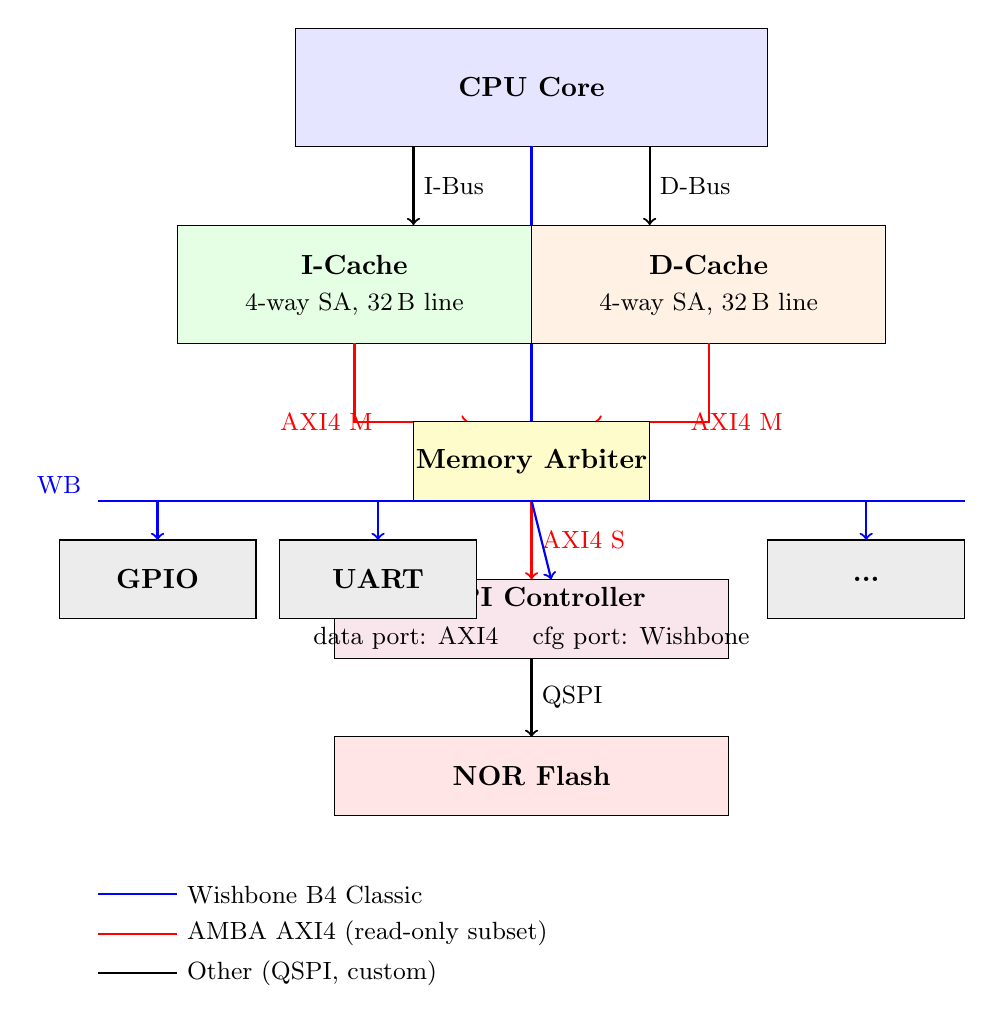
\begin{tikzpicture}[x=1cm, y=1cm]

  % ---- CPU Core ----
  \filldraw[fill=blue!10, draw=black] (3.0,13.0) rectangle (9.0,14.5);
  \node[align=center] at (6.0,13.75) {\textbf{CPU Core}};

  % I-Bus and D-Bus (custom, to caches)
  \draw[thick,->] (4.5,13.0) -- (4.5,12.0) node[midway,right,font=\small]{I-Bus};
  \draw[thick,->] (7.5,13.0) -- (7.5,12.0) node[midway,right,font=\small]{D-Bus};

  % Wishbone master port (CPU downward to WB bus)
  \draw[thick,blue,->] (6.0,13.0) -- (6.0,8.5)
    node[midway,left,font=\small,blue]{Wishbone};

  % ---- I-Cache ----
  \filldraw[fill=green!10, draw=black] (1.5,10.5) rectangle (6.0,12.0);
  \node[align=center] at (3.75,11.5) {\textbf{I-Cache}};
  \node[align=center,font=\small] at (3.75,11.0) {4-way SA, 32\,B line};

  % ---- D-Cache ----
  \filldraw[fill=orange!10, draw=black] (6.0,10.5) rectangle (10.5,12.0);
  \node[align=center] at (8.25,11.5) {\textbf{D-Cache}};
  \node[align=center,font=\small] at (8.25,11.0) {4-way SA, 32\,B line};

  % AXI4 from I-Cache to arbiter
  \draw[thick,red,->] (3.75,10.5) -- (3.75,9.5) -- (5.2,9.5)
    node[near start,left,font=\small,red]{AXI4 M};

  % AXI4 from D-Cache to arbiter
  \draw[thick,red,->] (8.25,10.5) -- (8.25,9.5) -- (6.8,9.5)
    node[near start,right,font=\small,red]{AXI4 M};

  % ---- Memory Arbiter ----
  \filldraw[fill=yellow!20, draw=black] (4.5,8.5) rectangle (7.5,9.5);
  \node[align=center] at (6.0,9.0) {\textbf{Memory Arbiter}};

  % AXI4 from arbiter to QSPI
  \draw[thick,red,->] (6.0,8.5) -- (6.0,7.5)
    node[midway,right,font=\small,red]{AXI4 S};

  % ---- QSPI Controller ----
  \filldraw[fill=purple!10, draw=black] (3.5,6.5) rectangle (8.5,7.5);
  \node[align=center] at (6.0,7.25) {\textbf{QSPI Controller}};
  \node[align=center,font=\small] at (6.0,6.75) {data port: AXI4 \quad cfg port: Wishbone};

  % Wishbone to QSPI cfg port
  \draw[thick,blue,->] (6.0,8.5) -- (6.25,7.5);

  % QSPI bus to NOR Flash
  \draw[thick,->] (6.0,6.5) -- (6.0,5.5) node[midway,right,font=\small]{QSPI};

  % ---- NOR Flash ----
  \filldraw[fill=red!10, draw=black] (3.5,4.5) rectangle (8.5,5.5);
  \node[align=center] at (6.0,5.0) {\textbf{NOR Flash}};

  % ---- Wishbone Bus ----
  \draw[thick,blue] (0.5,8.5) -- (11.5,8.5);
  \node[blue,font=\small] at (0.0,8.7) {WB};

  % ---- GPIO ----
  \filldraw[fill=gray!15, draw=black] (0.0,7.0) rectangle (2.5,8.0);
  \node[align=center] at (1.25,7.5) {\textbf{GPIO}};
  \draw[thick,blue,->] (1.25,8.5) -- (1.25,8.0);

  % ---- UART ----
  \filldraw[fill=gray!15, draw=black] (2.8,7.0) rectangle (5.3,8.0);
  \node[align=center] at (4.05,7.5) {\textbf{UART}};
  \draw[thick,blue,->] (4.05,8.5) -- (4.05,8.0);

  % ---- ... ----
  \filldraw[fill=gray!15, draw=black] (9.0,7.0) rectangle (11.5,8.0);
  \node[align=center] at (10.25,7.5) {\textbf{...}};
  \draw[thick,blue,->] (10.25,8.5) -- (10.25,8.0);

  % Legend
  \draw[thick,blue] (0.5,3.5) -- (1.5,3.5);
  \node[right,font=\small] at (1.5,3.5) {Wishbone B4 Classic};
  \draw[thick,red]  (0.5,3.0) -- (1.5,3.0);
  \node[right,font=\small] at (1.5,3.0) {AMBA AXI4 (read-only subset)};
  \draw[thick]      (0.5,2.5) -- (1.5,2.5);
  \node[right,font=\small] at (1.5,2.5) {Other (QSPI, custom)};

\end{tikzpicture}
\caption{On-Chip Bus Topology -- Dual-Bus Architecture}
\label{fig:asBusTopology}
\end{figure}

%%%%%%%%%%%%%%%%%%%%%%%%%%%%%%%%%%%%%%%%%%%%%%%%%%%%%%%%%%%%%%%%%%%%%%%%%%%%%
\subsection{Bus Selection Rationale}
\label{subsec:asBusRationale}
%%%%%%%%%%%%%%%%%%%%%%%%%%%%%%%%%%%%%%%%%%%%%%%%%%%%%%%%%%%%%%%%%%%%%%%%%%%%%

Table~\ref{tab:asBusRationale} documents the decision to use a dual-bus
architecture rather than a single unified bus for all on-chip traffic.

\begin{table}[H]
\caption{Bus Selection Rationale}
\label{tab:asBusRationale}
\centering
\begin{tabularx}{\textwidth}{|l |X |X|}
  \hline
  Criterion & Wishbone (peripherals) & AXI4 (cache) \\
  \hline
  \hline
  Transfer pattern &
    Single register read/write; one word per transaction &
    32-byte cache line fill; 4 beats per transaction \\
  \hline
  Burst support &
    Not needed; register accesses are always single-word &
    Essential; without bursts, 8 independent transactions per
    cache miss instead of 1 \\
  \hline
  Latency &
    Zero wait states (combinatorial ACK); adequate for
    register accesses &
    Many cycles per miss; decoupled AR and R channels
    allow the QSPI controller to accept the address and
    then stream data without stalling the bus \\
  \hline
  Complexity &
    Very simple; no state machines required in the BPI &
    Higher; separate address/data channels, handshaking,
    ID tracking -- justified by the burst benefit \\
  \hline
  IP compatibility &
    All existing peripheral IP blocks use Wishbone;
    no changes required &
    Cache controllers are new IP; designed for AXI4 from
    the start \\
  \hline
  Write support &
    Full read/write (register access) &
    Read-only (write channels eliminated by MEM-01
    resolution; Flash is read-only) \\
  \hline
  Decision &
    \textbf{Keep Wishbone for all peripherals.}
    Adding AXI4 to GPIO/UART etc.\ would add complexity
    with no benefit. &
    \textbf{Use AXI4 for cache--memory path.}
    The 8$\times$ reduction in bus transactions per cache
    miss justifies the added complexity. \\
  \hline
\end{tabularx}
\end{table}

%%%%%%%%%%%%%%%%%%%%%%%%%%%%%%%%%%%%%%%%%%%%%%%%%%%%%%%%%%%%%%%%%%%%%%%%%%%%%
\subsection{Wishbone B4 Classic -- Peripheral Bus}
%%%%%%%%%%%%%%%%%%%%%%%%%%%%%%%%%%%%%%%%%%%%%%%%%%%%%%%%%%%%%%%%%%%%%%%%%%%%%

\subsubsection{Signal Naming Convention}

Wishbone signal names in this design follow the convention shown in
Table~\ref{tab:asBusConcept02}.
The suffix \texttt{\_i} indicates an input, \texttt{\_o} an output,
and \texttt{\_s} an internal wire.
The prefix \texttt{wb\_s\_} is used for slave-side signals and
\texttt{wb\_m\_} for master-side signals.

\begin{table}[H]
\caption{Wishbone Signal Naming}
\label{tab:asBusConcept02}
\centering
\begin{tabularx}{\textwidth}{|l |l |l |l |X|}
  \hline
  Wishbone Name & Slave Port & Master Port & Width & Description \\
  \hline
  \hline
  ADR    & \texttt{wb\_s\_addr\_i} & \texttt{wb\_m\_addr\_o} & 64 & Address bus \\
  \hline
  DAT\_I & \texttt{wb\_s\_dat\_i}  & \texttt{wb\_m\_dat\_i}  & 64 & Data from master to slave (write data) \\
  \hline
  DAT\_O & \texttt{wb\_s\_dat\_o}  & \texttt{wb\_m\_dat\_o}  & 64 & Data from slave to master (read data) \\
  \hline
  WE     & \texttt{wb\_s\_we\_i}   & \texttt{wb\_m\_we\_o}   & 1  & Write enable: 1 = write, 0 = read \\
  \hline
  SEL    & \texttt{wb\_s\_sel\_i}  & \texttt{wb\_m\_sel\_o}  & 8  & Byte select (all bytes must be set) \\
  \hline
  STB    & \texttt{wb\_s\_stb\_i}  & \texttt{wb\_m\_stb\_o}  & 1  & Strobe: valid cycle indicator from master \\
  \hline
  ACK    & \texttt{wb\_s\_ack\_o}  & \texttt{wb\_m\_ack\_i}  & 1  & Acknowledge: normal end of transfer from slave \\
  \hline
  CYC    & \texttt{wb\_s\_cyc\_i}  & \texttt{wb\_m\_cyc\_o}  & 1  & Cycle: bus cycle active (held for complete transfer) \\
  \hline
\end{tabularx}
\end{table}

\subsubsection{Transfer Protocol}

A Wishbone Classic single transfer proceeds as follows:

\begin{enumerate}
  \item The master asserts \texttt{CYC} and \texttt{STB}, presents a valid
    address on \texttt{ADR}, drives \texttt{WE} (1 for write, 0 for read),
    sets \texttt{SEL} to all-ones, and -- for a write -- provides data on
    \texttt{DAT\_O}.
  \item In this implementation the slave responds \emph{combinatorially} in the
    same clock cycle: it drives read data on \texttt{DAT\_O} and asserts
    \texttt{ACK}.
  \item The transaction is complete when both \texttt{STB} and \texttt{ACK}
    are seen high on the rising clock edge.
    The master may then begin a new transfer in the very next cycle.
\end{enumerate}

A transfer is considered valid only when both \texttt{CYC} and \texttt{STB}
are asserted simultaneously and all byte-select bits are set.
If any byte-select bit is clear the BPI treats the access as invalid and
suppresses both the ACK and the write enable to the peripheral.

The timing diagram below illustrates a write followed by a read.

\begin{figure}[H]
\centering
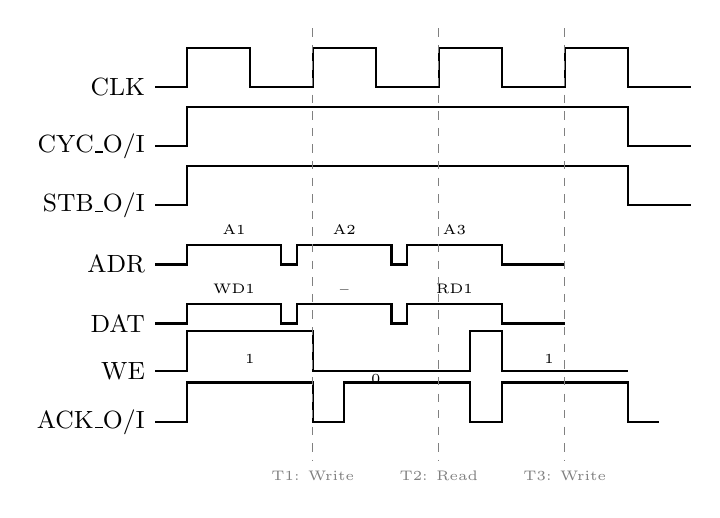
\begin{tikzpicture}[x=0.8cm, y=0.5cm]
  % Clock
  \draw[thick] (0,8) node[left]{\small CLK}
    -- ++(0.5,0) -- ++(0,1) -- ++(1,0) -- ++(0,-1) -- ++(1,0) -- ++(0,1) -- ++(1,0) -- ++(0,-1)
    -- ++(1,0) -- ++(0,1) -- ++(1,0) -- ++(0,-1) -- ++(1,0) -- ++(0,1) -- ++(1,0) -- ++(0,-1) -- ++(1,0);
  % CYC
  \draw[thick] (0,6.5) node[left]{\small CYC\_O/I}
    -- ++(0.5,0) -- ++(0,1) -- ++(7,0) -- ++(0,-1) -- ++(1,0);
  % STB
  \draw[thick] (0,5) node[left]{\small STB\_O/I}
    -- ++(0.5,0) -- ++(0,1) -- ++(7,0) -- ++(0,-1) -- ++(1,0);
  % ADR (two phases)
  \draw[thick] (0,3.5) node[left]{\small ADR}
    -- ++(0.5,0)
    -- ++(0,0.5) -- ++(1.5,0) node[midway,above]{\tiny A1}
    -- ++(0,-0.5) -- ++(0.25,0) -- ++(0,0.5)
    -- ++(1.5,0) node[midway,above]{\tiny A2}
    -- ++(0,-0.5) -- ++(0.25,0) -- ++(0,0.5)
    -- ++(1.5,0) node[midway,above]{\tiny A3}
    -- ++(0,-0.5) -- ++(1,0);
  % DAT (write, then read)
  \draw[thick] (0,2) node[left]{\small DAT}
    -- ++(0.5,0)
    -- ++(0,0.5) -- ++(1.5,0) node[midway,above]{\tiny WD1}
    -- ++(0,-0.5) -- ++(0.25,0) -- ++(0,0.5)
    -- ++(1.5,0) node[midway,above]{\tiny --}
    -- ++(0,-0.5) -- ++(0.25,0) -- ++(0,0.5)
    -- ++(1.5,0) node[midway,above]{\tiny RD1}
    -- ++(0,-0.5) -- ++(1,0);
  % WE
  \draw[thick] (0,0.8) node[left]{\small WE}
    -- ++(0.5,0) -- ++(0,1) -- ++(2,0) -- ++(0,-1) -- ++(2.5,0) -- ++(0,1) -- ++(0.5,0) -- ++(0,-1)  -- ++(2,0);
  \node at (1.5,1.1)  {\tiny 1};
  \node at (3.5,0.6)  {\tiny 0};
  \node at (6.25,1.1) {\tiny 1};
  % ACK
  \draw[thick] (0,-0.5) node[left]{\small ACK\_O/I}
    -- ++(0.5,0) -- ++(0,1) -- ++(2,0) -- ++(0,-1)
    -- ++(0.5,0) -- ++(0,1) -- ++(2,0) -- ++(0,-1)
    -- ++(0.5,0) -- ++(0,1) -- ++(2,0) -- ++(0,-1) -- ++(0.5,0);
  % Labels
  \draw[dashed,gray] (2.5,9.5) -- (2.5,-1.5) node[below]{\tiny T1: Write};
  \draw[dashed,gray] (4.5,9.5) -- (4.5,-1.5) node[below]{\tiny T2: Read};
  \draw[dashed,gray] (6.5,9.5) -- (6.5,-1.5) node[below]{\tiny T3: Write};
\end{tikzpicture}
\caption{Wishbone Classic Single Transfers: Write -- Read -- Write}
\label{fig:asBusTiming01}
\end{figure}

\subsubsection{Byte Select}

The 8-bit \texttt{SEL} signal indicates which byte lanes carry valid data.
Bit\;$n$ of \texttt{SEL} corresponds to byte lane\;$n$ (bits $8n+7\ldots 8n$)
of the 64-bit data bus.
In the current implementation, the master BPI always drives all eight
\texttt{SEL} bits to~1 (full-word transfers only).
The slave BPI checks that all \texttt{SEL} bits are set before asserting
\texttt{ACK} or issuing a write enable to the peripheral kernel.
Sub-word accesses are therefore not supported.

\subsubsection{Reset Behaviour}

All Wishbone outputs are driven to their inactive state while the synchronous
active-high reset \texttt{rst\_i} is asserted.
For the master BPI this means \texttt{STB\_O} and \texttt{CYC\_O} are held
low; for the slave BPI \texttt{ACK\_O} is held low.
Note that in the current purely combinatorial implementation the reset
is not registered inside the BPI modules; the reset is applied by the
surrounding peripheral logic.

%%%%%%%%%%%%%%%%%%%%%%%%%%%%%%%%%%%%%%%%%%%%%%%%%%%%%%%%%%%%%%%%%%%%%%%%%%%%%
\subsection{AMBA AXI4 -- Cache Memory Bus}
\label{subsec:asAxi4Bus}
%%%%%%%%%%%%%%%%%%%%%%%%%%%%%%%%%%%%%%%%%%%%%%%%%%%%%%%%%%%%%%%%%%%%%%%%%%%%%

\subsubsection{Overview}

The AXI4 bus connects the two cache controllers (I-Cache and D-Cache)
through the Memory Arbiter to the QSPI controller data port.
It carries exclusively 32-byte cache-line read bursts.
Write channels (AW, W, B) are not instantiated: the AXI4 write path was
eliminated when the scratchpad SRAM replaced write-back-to-Flash
(MEM-01 resolution).

\subsubsection{Participants}

\begin{table}[H]
\caption{AXI4 Bus Participants}
\label{tab:asAxi4Participants}
\centering
\begin{tabularx}{\textwidth}{|l |l |X|}
  \hline
  Block & Role & Notes \\
  \hline
  \hline
  I-Cache controller & AXI4 Master (ID=0x1) &
    Issues read burst on cache miss; read-only \\
  \hline
  D-Cache controller & AXI4 Master (ID=0x2) &
    Issues read burst on cache miss; read-only \\
  \hline
  Memory Arbiter     & AXI4 Slave + Master &
    Accepts two masters; forwards one at a time to QSPI;
    fixed priority D-Cache $>$ I-Cache \\
  \hline
  QSPI controller (data port) & AXI4 Slave &
    Translates AXI4 read burst to Quad Fast Read SPI command;
    slow slave (many cycles per burst) \\
  \hline
\end{tabularx}
\end{table}

\subsubsection{Bus Parameters}

The AXI4 bus uses a reduced parameter set:
all transfers are fixed-length 4-beat INCR read bursts.

\begin{table}[H]
\caption{AXI4 Cache Bus Parameters}
\label{tab:asAxi4BusParams}
\centering
\begin{tabularx}{\textwidth}{|l |l |X|}
  \hline
  Parameter & Value & Comment \\
  \hline
  \hline
  Protocol       & AXI4 (not AXI4-Lite)   & Burst support required \\
  \hline
  Data width     & 64\,bit                 & One RV64 doubleword per beat \\
  \hline
  Address width  & 32\,bit                 & Physical address (\texttt{PA\_WIDTH=32}) \\
  \hline
  ID width       & 4\,bit                  & I-Cache: \texttt{4'h1}; D-Cache: \texttt{4'h2} \\
  \hline
  Burst type     & INCR only               & Sequential address; no WRAP, no FIXED \\
  \hline
  Burst length   & ARLEN = 3               & 4 beats $\times$ 8\,B = 32\,B per cache line \\
  \hline
  Beat size      & ARSIZE = 3              & 8 bytes per beat \\
  \hline
  Channels used  & AR, R only              & AW, W, B channels not instantiated \\
  \hline
  Outstanding tx & 1 per master            & Each cache has at most 1 transaction in flight \\
  \hline
\end{tabularx}
\end{table}

The full AXI4 channel signal definitions, the SystemVerilog interface
\texttt{as\_axi4\_if}, and the AXI4 timing diagrams are documented in
the Memory Concept section (Section~``Memory Concept'',
subsection ``AXI4 Memory Bus'').

\subsubsection{QSPI Controller -- Dual Bus Participation}

The QSPI controller is the only block that participates in both buses:

\begin{itemize}
  \item \textbf{AXI4 slave port (data):}
    Receives 4-beat INCR read bursts from the Memory Arbiter.
    Translates each burst into a Quad Fast Read (\texttt{0x6B})
    command sequence on the SPI bus and returns 32 bytes in 4 AXI4
    R-channel beats.
    This port is part of the AXI4 cache memory bus.

  \item \textbf{Wishbone slave port (configuration):}
    Receives single-word register accesses from the CPU for
    QSPI mode configuration, status readback, and manual SPI command
    injection.
    This port is part of the Wishbone peripheral bus and uses the
    standard \texttt{as\_slave\_bpi} wrapper.
\end{itemize}

The two ports are independent and may be active simultaneously.
The QSPI controller arbitrates internally between the AXI4 data path
and the Wishbone configuration path, with the AXI4 burst taking
priority over a concurrent Wishbone access.

%%%%%%%%%%%%%%%%%%%%%%%%%%%%%%%%%%%%%%%%%%%%%%%%%%%%%%%%%%%%%%%%%%%%%%%%%%%%%
\subsection{Wishbone Slave BPI (\texttt{as\_slave\_bpi})}
\label{subsec:asSlaveBpi}
%%%%%%%%%%%%%%%%%%%%%%%%%%%%%%%%%%%%%%%%%%%%%%%%%%%%%%%%%%%%%%%%%%%%%%%%%%%%%

\subsubsection{History}
\begin{table}[H]
\caption{History of as\_slave\_bpi}
\label{tab:asSlaveBpiHist}
\centering
\begin{tabularx}{\textwidth}{|l |l |l |X|}
  \hline
  Version & Date & Author & Change \\
  \hline
  \hline
  0.1 & 2026-02-19 & Claude-AI & Initial version, Wishbone B4 Classic, zero wait states \\
  \hline
\end{tabularx}
\end{table}

\subsubsection{Functional Configuration of as\_slave\_bpi}

The \texttt{as\_slave\_bpi} module implements the Wishbone B4 Classic
slave interface.
It converts Wishbone bus signals into simple register-file read and write
enables for the peripheral kernel.
Table~\ref{tab:asSlaveBpiCfg} lists the configurable parameters.

\begin{table}[H]
\caption{Functional Configuration of as\_slave\_bpi}
\label{tab:asSlaveBpiCfg}
\centering
\begin{tabularx}{\textwidth}{|l |l |l |X|}
  \hline
  Parameter & Type & Default & Description \\
  \hline
  \hline
  \texttt{addr\_width} & integer & 64 & Width of the address bus in bits \\
  \hline
  \texttt{data\_width} & integer & 64 & Width of the data bus in bits; also determines SEL width as \texttt{data\_width/8} \\
  \hline
\end{tabularx}
\end{table}

\subsubsection{HW Interfaces}

Table~\ref{tab:asSlaveBpiIO} lists all input and output ports of the
\texttt{as\_slave\_bpi} module.

\begin{table}[H]
\caption{I/O of as\_slave\_bpi}
\label{tab:asSlaveBpiIO}
\centering
\begin{tabularx}{\textwidth}{|l |l |l |X|}
  \hline
  Port & Direction & Width & Description \\
  \hline
  \hline
  \texttt{rst\_i}            & in  & 1  & Synchronous reset, active high \\
  \hline
  \texttt{clk\_i}            & in  & 1  & Bus clock \\
  \hline
  \multicolumn{4}{|l|}{Peripheral kernel side:} \\
  \hline
  \texttt{addr\_o}           & out & 64 & Decoded register address to peripheral \\
  \hline
  \texttt{dat\_from\_core\_i}& in  & 64 & Read data returned by peripheral kernel \\
  \hline
  \texttt{dat\_to\_core\_o}  & out & 64 & Write data forwarded to peripheral kernel \\
  \hline
  \texttt{wr\_o}             & out & 1  & Write enable to peripheral: asserted for one cycle on a valid write \\
  \hline
  \texttt{rd\_o}             & out & 1  & Read enable to peripheral: asserted for one cycle on a valid read \\
  \hline
  \multicolumn{4}{|l|}{Wishbone bus side:} \\
  \hline
  \texttt{wb\_s\_addr\_i}    & in  & 64 & Address from Wishbone master \\
  \hline
  \texttt{wb\_s\_dat\_i}     & in  & 64 & Write data from Wishbone master \\
  \hline
  \texttt{wb\_s\_dat\_o}     & out & 64 & Read data to Wishbone master \\
  \hline
  \texttt{wb\_s\_we\_i}      & in  & 1  & Write enable from Wishbone master \\
  \hline
  \texttt{wb\_s\_sel\_i}     & in  & 8  & Byte select from Wishbone master \\
  \hline
  \texttt{wb\_s\_stb\_i}     & in  & 1  & Strobe from Wishbone master \\
  \hline
  \texttt{wb\_s\_ack\_o}     & out & 1  & Acknowledge to Wishbone master \\
  \hline
  \texttt{wb\_s\_cyc\_i}     & in  & 1  & Cycle from Wishbone master \\
  \hline
\end{tabularx}
\end{table}

\subsubsection{Bus Interface}

Wishbone Classic Slave.

\subsubsection{Registers}

The \texttt{as\_slave\_bpi} module contains no registers of its own.
All logic is purely combinatorial.
Registers are located in the peripheral kernel that is connected via the
kernel-side interface of this module.

\subsubsection{Related Sections of this Specification}

\begin{itemize}
  \item Wishbone Master BPI Section~\ref{subsec:asMasterBpi}
  \item QSPI Peripheral Section~\ref{sec:qspifunc01}, which uses this BPI
  \item GPIO Peripheral Section~\ref{sec:gpiofunc01}, which uses this BPI
\end{itemize}

\subsubsection{Functional Overview}

The slave BPI converts two Wishbone control signals plus the byte-select
into two conditions used throughout the peripheral:

\[
  \textit{valid\_transfer} = \texttt{CYC} \;\land\; \texttt{STB}
\]
\[
  \textit{all\_sel} = \&\;\texttt{SEL}_{7:0}
\]

From these two conditions the write and read enables to the peripheral
kernel are derived:

\[
  \texttt{wr\_o} = \textit{valid\_transfer} \;\land\; \texttt{WE} \;\land\; \textit{all\_sel}
\]
\[
  \texttt{rd\_o} = \textit{valid\_transfer} \;\land\; \lnot\texttt{WE} \;\land\; \textit{all\_sel}
\]

The Wishbone acknowledge is generated combinatorially:

\[
  \texttt{ACK\_O} = \textit{valid\_transfer} \;\land\; \textit{all\_sel}
\]

Because ACK is driven combinatorially from STB and CYC, the slave
introduces zero wait states.
The peripheral kernel must therefore provide read data (\texttt{dat\_from\_core\_i})
in the same clock cycle that \texttt{rd\_o} is asserted.

\subsubsection{Structural Overview}

Figure~\ref{fig:asSlaveBpi01} shows the internal signal flow of the slave BPI.

\begin{figure}[H]
\centering
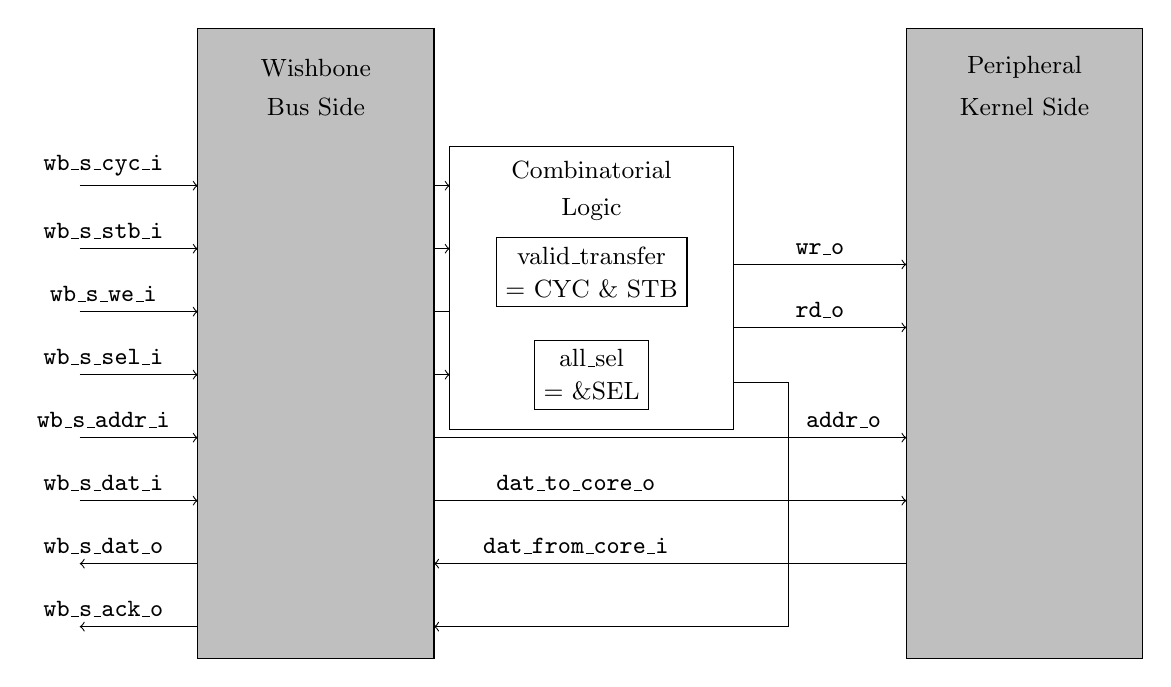
\begin{tikzpicture}
  % Bus-side box (left)
  \filldraw[fill=lightgray, draw=black] (0,0) rectangle (3,8);
  \node[align=center] at (1.5,7.5) {\small Wishbone};
  \node[align=center] at (1.5,7.0) {\small Bus Side};
  % Bus inputs
  \draw[->] (-1.5,6.0) -- (0,6.0) node[above,yshift=0.0cm,xshift=-1.2cm]{\small \texttt{wb\_s\_cyc\_i}};
  \draw[->] (-1.5,5.2) -- (0,5.2) node[above,yshift=0.0cm,xshift=-1.2cm]{\small \texttt{wb\_s\_stb\_i}};
  \draw[->] (-1.5,4.4) -- (0,4.4) node[above,yshift=0.0cm,xshift=-1.2cm]{\small \texttt{wb\_s\_we\_i}};
  \draw[->] (-1.5,3.6) -- (0,3.6) node[above,yshift=0.0cm,xshift=-1.2cm]{\small \texttt{wb\_s\_sel\_i}};
  \draw[->] (-1.5,2.8) -- (0,2.8) node[above,yshift=0.0cm,xshift=-1.2cm]{\small \texttt{wb\_s\_addr\_i}};
  \draw[->] (-1.5,2.0) -- (0,2.0) node[above,yshift=0.0cm,xshift=-1.2cm]{\small \texttt{wb\_s\_dat\_i}};
  \draw[<-] (-1.5,1.2) -- (0,1.2) node[above,yshift=0.0cm,xshift=-1.2cm]{\small \texttt{wb\_s\_dat\_o}};
  \draw[<-] (-1.5,0.4) -- (0,0.4) node[above,yshift=0.0cm,xshift=-1.2cm]{\small \texttt{wb\_s\_ack\_o}};
  % Logic box (centre)
  \filldraw[fill=white, draw=black] (3.2,2.9) rectangle (6.8,6.5);
  \node[align=center] at (5,6.2) {\small Combinatorial};
  \node[align=center] at (5,5.7) {\small Logic};
  % AND gate label
  \node[draw,align=center,fill=white] at (5,4.9) {\small valid\_transfer\\ \small = CYC \& STB};
  \node[draw,align=center,fill=white] at (5,3.6) {\small all\_sel\\ \small = \&SEL};
  % Connections bus→logic
  \draw[->] (3,6.0) -- (3.2,6);
  \draw[->] (3,5.2) -- (3.2,5.2);
  \draw[-]  (3,4.4) -- (3.2,4.4);
  \draw[->] (3,3.6) -- (3.2,3.6);
  % Kernel-side box (right)
  \filldraw[fill=lightgray, draw=black] (9,0) rectangle (12,8);
  \node[align=center] at (10.5,7.5) {\small Peripheral};
  \node[align=center] at (10.5,7.0) {\small Kernel Side};
  % addr passthrough
  \draw[->] (3,2.8) -- (9,2.8) node[midway,above, xshift=2.2cm]{\small \texttt{addr\_o}};
  % write data passthrough
  \draw[->] (3,2.0) -- (9,2.0) node[midway,above, xshift=-1.2cm]{\small \texttt{dat\_to\_core\_o}};
  % read data passthrough
  \draw[<-] (3,1.2) -- (9,1.2) node[midway,above, xshift=-1.2cm]{\small \texttt{dat\_from\_core\_i}};
  % wr_o from logic
  \draw[->] (6.8,5.0) -- (9,5.0) node[midway,above]{\small \texttt{wr\_o}};
  % rd_o from logic
  \draw[->] (6.8,4.2) -- (9,4.2) node[midway,above]{\small \texttt{rd\_o}};
  % ack_o back to bus
  \draw[->] (6.8,3.5) -- (7.5,3.5) -- (7.5,0.4) -- (3,0.4);
\end{tikzpicture}
\caption{as\_slave\_bpi -- Internal Signal Flow}
\label{fig:asSlaveBpi01}
\end{figure}

Table~\ref{tab:asSlaveBpiInt} lists the internal signals.

\begin{table}[H]
\caption{as\_slave\_bpi Internal Signals}
\label{tab:asSlaveBpiInt}
\centering
\begin{tabularx}{\textwidth}{|l |l |l |X|}
  \hline
  Signal & Type & Width & Description \\
  \hline
  \hline
  \texttt{valid\_transfer\_s} & logic & 1 & High when both CYC and STB are asserted.
    Indicates an active Wishbone bus cycle. \\
  \hline
  \texttt{all\_sel\_s}        & logic & 1 & High when all byte-select bits are set.
    Only full 64-bit word accesses are accepted. \\
  \hline
\end{tabularx}
\end{table}

\subsubsection{Instantiation}

The module is parameterised and instantiated as follows:

\begin{verbatim}
as_slave_bpi #(
    .addr_width ( 64 ),
    .data_width ( 64 )
) u_qspi_bpi (
    .rst_i              ( rst_i              ),
    .clk_i              ( clk_i              ),
    // kernel side
    .addr_o             ( addr_s             ),
    .dat_from_core_i    ( dat_from_core_s    ),
    .dat_to_core_o      ( dat_to_core_s      ),
    .wr_o               ( wr_s               ),
    .rd_o               ( rd_s               ),
    // wishbone side
    .wb_s_addr_i        ( wb_s_addr_i        ),
    .wb_s_dat_i         ( wb_s_dat_i         ),
    .wb_s_dat_o         ( wb_s_dat_o         ),
    .wb_s_we_i          ( wb_s_we_i          ),
    .wb_s_sel_i         ( wb_s_sel_i         ),
    .wb_s_stb_i         ( wb_s_stb_i         ),
    .wb_s_ack_o         ( wb_s_ack_o         ),
    .wb_s_cyc_i         ( wb_s_cyc_i         )
);
\end{verbatim}

\subsubsection{Limitations and Design Rules}

\begin{itemize}
  \item \textbf{Zero wait states only.}
    The peripheral kernel must provide read data combinatorially.
    If the kernel uses registered outputs, a wait-state mechanism
    (delayed ACK) must be added externally.
  \item \textbf{Full-word accesses only.}
    Sub-word byte or half-word accesses are not supported.
    The \texttt{SEL} check ensures that partial accesses are rejected silently.
  \item \textbf{No ERR\_O.}
    Bus errors are not signalled. Invalid accesses are simply not acknowledged
    (ACK stays low).
  \item \textbf{No burst support.}
    The module supports only Wishbone Classic single-cycle transfers.
    Pipeline or burst modes are not implemented.
  \item \textbf{Combinatorial ACK.}
    Connecting multiple slave BPIs in a shared-bus topology requires
    that ACK is only driven by the selected slave. Address decoding
    and ACK gating must be handled by the bus interconnect logic, not
    by this module.
\end{itemize}


%%%%%%%%%%%%%%%%%%%%%%%%%%%%%%%%%%%%%%%%%%%%%%%%%%%%%%%%%%%%%%%%%%%%%%%%%%%%%
\subsection{Wishbone Master BPI (\texttt{as\_master\_bpi})}
\label{subsec:asMasterBpi}
%%%%%%%%%%%%%%%%%%%%%%%%%%%%%%%%%%%%%%%%%%%%%%%%%%%%%%%%%%%%%%%%%%%%%%%%%%%%%

\subsubsection{History}
\begin{table}[H]
\caption{History of as\_master\_bpi}
\label{tab:asMasterBpiHist}
\centering
\begin{tabularx}{\textwidth}{|l |l |l |X|}
  \hline
  Version & Date & Author & Change \\
  \hline
  \hline
  0.1 & 2026-02-19 & Claude-AI & Initial version, Wishbone B4 Classic, continuous CYC/STB \\
  \hline
\end{tabularx}
\end{table}

\subsubsection{Functional Configuration of as\_master\_bpi}

The \texttt{as\_master\_bpi} module implements the Wishbone B4 Classic
master interface.
It is a simple combinatorial wrapper that translates address, data and
direction signals from the CPU or DMA core into Wishbone master signals.
Table~\ref{tab:asMasterBpiCfg} lists the configurable parameters.

\begin{table}[H]
\caption{Functional Configuration of as\_master\_bpi}
\label{tab:asMasterBpiCfg}
\centering
\begin{tabularx}{\textwidth}{|l |l |l |X|}
  \hline
  Parameter & Type & Default & Description \\
  \hline
  \hline
  \texttt{addr\_width} & integer & 64 & Width of the address bus in bits \\
  \hline
  \texttt{data\_width} & integer & 64 & Width of the data bus in bits; also determines SEL width as \texttt{data\_width/8} \\
  \hline
\end{tabularx}
\end{table}

\subsubsection{HW Interfaces}

Table~\ref{tab:asMasterBpiIO} lists all input and output ports of the
\texttt{as\_master\_bpi} module.

\begin{table}[H]
\caption{I/O of as\_master\_bpi}
\label{tab:asMasterBpiIO}
\centering
\begin{tabularx}{\textwidth}{|l |l |l |X|}
  \hline
  Port & Direction & Width & Description \\
  \hline
  \hline
  \texttt{rst\_i}             & in  & 1  & Synchronous reset, active high \\
  \hline
  \texttt{clk\_i}             & in  & 1  & Bus clock \\
  \hline
  \multicolumn{4}{|l|}{CPU / master core side:} \\
  \hline
  \texttt{addr\_i}            & in  & 64 & Address from CPU core \\
  \hline
  \texttt{dat\_from\_core\_i} & in  & 64 & Write data from CPU core \\
  \hline
  \texttt{dat\_to\_core\_o}   & out & 64 & Read data returned to CPU core \\
  \hline
  \texttt{wr\_i}              & in  & 1  & Write enable from CPU core: 1 = write, 0 = read \\
  \hline
  \multicolumn{4}{|l|}{Wishbone bus side:} \\
  \hline
  \texttt{wb\_m\_addr\_o}     & out & 64 & Address to Wishbone bus \\
  \hline
  \texttt{wb\_m\_dat\_i}      & in  & 64 & Read data from Wishbone bus (from selected slave) \\
  \hline
  \texttt{wb\_m\_dat\_o}      & out & 64 & Write data to Wishbone bus \\
  \hline
  \texttt{wb\_m\_we\_o}       & out & 1  & Write enable to Wishbone bus \\
  \hline
  \texttt{wb\_m\_sel\_o}      & out & 8  & Byte select to Wishbone bus (always all-ones) \\
  \hline
  \texttt{wb\_m\_stb\_o}      & out & 1  & Strobe to Wishbone bus (tied high) \\
  \hline
  \texttt{wb\_m\_ack\_i}      & in  & 1  & Acknowledge from Wishbone bus (from selected slave) \\
  \hline
  \texttt{wb\_m\_cyc\_o}      & out & 1  & Cycle to Wishbone bus (tied high) \\
  \hline
\end{tabularx}
\end{table}

\subsubsection{Bus Interface}

Wishbone Classic Master.

\subsubsection{Registers}

The \texttt{as\_master\_bpi} module contains no registers of its own.
All logic is purely combinatorial.

\subsubsection{Related Sections of this Specification}

\begin{itemize}
  \item Wishbone Slave BPI Section~\ref{subsec:asSlaveBpi}
  \item RWU-RV64I Core Chapter, Bus Interface subsection
\end{itemize}

\subsubsection{Functional Overview}

The master BPI is a thin combinatorial bridge.
All Wishbone master outputs are driven directly from the CPU core signals
without any registered state:

\begin{align*}
  \texttt{wb\_m\_addr\_o} &= \texttt{addr\_i} \\
  \texttt{wb\_m\_dat\_o}  &= \texttt{dat\_from\_core\_i} \\
  \texttt{wb\_m\_we\_o}   &= \texttt{wr\_i} \\
  \texttt{wb\_m\_sel\_o}  &= \texttt{8'hFF} \quad \text{(all bytes always valid)} \\
  \texttt{wb\_m\_stb\_o}  &= 1 \\
  \texttt{wb\_m\_cyc\_o}  &= 1 \\
  \texttt{dat\_to\_core\_o} &= \texttt{wb\_m\_dat\_i}
\end{align*}

Because \texttt{STB} and \texttt{CYC} are continuously asserted, a new
Wishbone transfer is initiated on every clock cycle as long as a slave is
present on the bus.
The transfer completes when the slave returns \texttt{ACK}.
In the zero-wait-state case (slave BPI also combinatorial), ACK arrives
in the same cycle as STB, so every clock cycle is a completed transfer.

The CPU core must handle the \texttt{ack\_i} signal to determine when a
read result is valid or when the next write can proceed.

\subsubsection{Structural Overview}

Figure~\ref{fig:asMasterBpi01} shows the internal signal flow of the master BPI.

\begin{figure}[H]
\centering
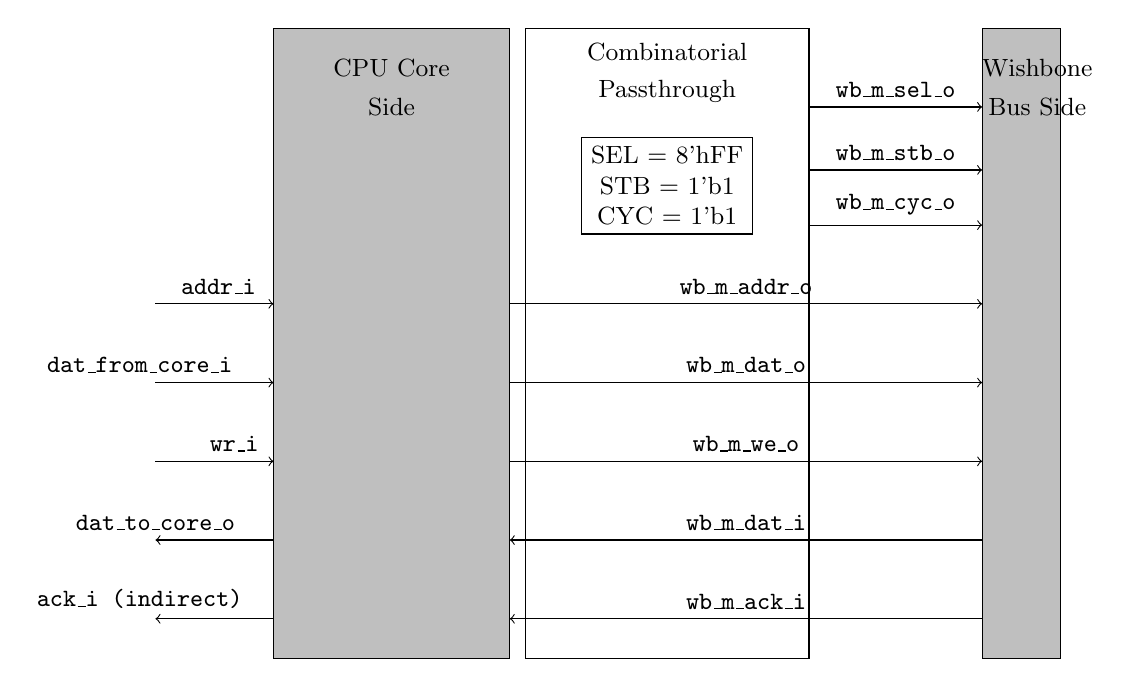
\begin{tikzpicture}
  % CPU/core side (left)
  \filldraw[fill=lightgray, draw=black] (0,0) rectangle (3,8);
  \node[align=center] at (1.5,7.5) {\small CPU Core};
  \node[align=center] at (1.5,7.0) {\small Side};
  % CPU inputs
  \draw[->] (-1.5,4.5) -- (0,4.5) node[left,above,xshift=-0.7cm]{\small \texttt{addr\_i}};
  \draw[->] (-1.5,3.5) -- (0,3.5) node[left,above,xshift=-1.7cm]{\small \texttt{dat\_from\_core\_i}};
  \draw[->] (-1.5,2.5) -- (0,2.5) node[left,above,xshift=-0.5cm]{\small \texttt{wr\_i}};
  \draw[<-] (-1.5,1.5) -- (0,1.5) node[left,above,xshift=-1.5cm]{\small \texttt{dat\_to\_core\_o}};
  \draw[<-] (-1.5,0.5) -- (0,0.5) node[left,above,xshift=-1.7cm]{\small \texttt{ack\_i (indirect)}};
  % Passthrough box (centre)
  \filldraw[fill=white, draw=black] (3.2,0.0) rectangle (6.8,8.0);
  \node[align=center] at (5,7.7) {\small Combinatorial};
  \node[align=center] at (5,7.2) {\small Passthrough};
  \node[draw,fill=white,align=center,font=\small] at (5,6.0)
    {SEL = 8'hFF \\ STB = 1'b1 \\ CYC = 1'b1};
  % Wishbone side (right)
  \filldraw[fill=lightgray, draw=black] (9,0) rectangle (10,8);
  \node[align=center] at (9.7,7.5) {\small Wishbone};
  \node[align=center] at (9.7,7.0) {\small Bus Side};
  % passthrough outputs
  \draw[->] (3,4.5) -- (9,4.5) node[midway,above]{\small \texttt{wb\_m\_addr\_o}};
  \draw[->] (3,3.5) -- (9,3.5) node[midway,above]{\small \texttt{wb\_m\_dat\_o}};
  \draw[->] (3,2.5) -- (9,2.5) node[midway,above]{\small \texttt{wb\_m\_we\_o}};
  \draw[<-] (3,1.5) -- (9,1.5) node[midway,above]{\small \texttt{wb\_m\_dat\_i}};
  \draw[<-] (3,0.5) -- (9,0.5) node[midway,above]{\small \texttt{wb\_m\_ack\_i}};
  % constant signals from logic box
  \draw[->] (6.8,7.0) -- (9,7.0) node[midway,above]{\small \texttt{wb\_m\_sel\_o}};
  \draw[->] (6.8,6.2) -- (9,6.2) node[midway,above]{\small \texttt{wb\_m\_stb\_o}};
  \draw[->] (6.8,5.5) -- (9,5.5) node[midway,above]{\small \texttt{wb\_m\_cyc\_o}};
\end{tikzpicture}
\caption{as\_master\_bpi -- Internal Signal Flow}
\label{fig:asMasterBpi01}
\end{figure}

Table~\ref{tab:asMasterBpiInt} lists the internal signals (none in this
implementation, as the module is purely combinatorial):

\begin{table}[H]
\caption{as\_master\_bpi Internal Signals}
\label{tab:asMasterBpiInt}
\centering
\begin{tabularx}{\textwidth}{|l |l |l |X|}
  \hline
  Signal & Type & Width & Description \\
  \hline
  \hline
  (none) & -- & -- & All logic is combinatorial; no internal signals \\
  \hline
\end{tabularx}
\end{table}

\subsubsection{Instantiation}

\begin{verbatim}
as_master_bpi #(
    .addr_width ( 64 ),
    .data_width ( 64 )
) u_cpu_bpi (
    .rst_i              ( rst_i              ),
    .clk_i              ( clk_i              ),
    // CPU core side
    .addr_i             ( cpu_addr_s         ),
    .dat_from_core_i    ( cpu_wdat_s         ),
    .dat_to_core_o      ( cpu_rdat_s         ),
    .wr_i               ( cpu_wr_s           ),
    // wishbone side
    .wb_m_addr_o        ( wb_m_addr_s        ),
    .wb_m_dat_i         ( wb_m_dat_i_s       ),
    .wb_m_dat_o         ( wb_m_dat_o_s       ),
    .wb_m_we_o          ( wb_m_we_s          ),
    .wb_m_sel_o         ( wb_m_sel_s         ),
    .wb_m_stb_o         ( wb_m_stb_s         ),
    .wb_m_ack_i         ( wb_m_ack_s         ),
    .wb_m_cyc_o         ( wb_m_cyc_s         )
);
\end{verbatim}

\subsubsection{Limitations and Design Rules}

\begin{itemize}
  \item \textbf{Continuous bus occupation.}
    Because \texttt{STB} and \texttt{CYC} are permanently asserted,
    the master occupies the bus at all times.
    Multi-master arbitration requires that these signals are gated
    by the arbiter before being placed on the shared bus.
  \item \textbf{No idle state.}
    The master BPI does not support idle cycles between transfers.
    The surrounding CPU core logic must insert idle cycles if needed
    by controlling \texttt{addr\_i} and \texttt{wr\_i} appropriately and
    ignoring any ACK responses during idle periods.
  \item \textbf{ACK not evaluated internally.}
    The \texttt{wb\_m\_ack\_i} signal is passed through directly to the
    CPU core via the bus-side port; the BPI itself does not act on it.
    The CPU must sample ACK and stall its pipeline if required.
  \item \textbf{No error handling.}
    There is no support for Wishbone \texttt{ERR\_I} or \texttt{RTY\_I}.
\end{itemize}


%%%%%%%%%%%%%%%%%%%%%%%%%%%%%%%%%%%%%%%%%%%%%%%%%%%%%%%%%%%%%%%%%%%%%%%%%%%%%
\subsection{Bus Interconnect}
\label{subsec:asBusInterconnect}
%%%%%%%%%%%%%%%%%%%%%%%%%%%%%%%%%%%%%%%%%%%%%%%%%%%%%%%%%%%%%%%%%%%%%%%%%%%%%

\subsubsection{Two Independent Buses}

The Wishbone and AXI4 buses are completely separate.
There is no bridge, no shared wires, and no arbitration between them.
Traffic routing is determined at design time by which port of each block
is connected to which bus:

\begin{itemize}
  \item All CPU accesses to peripheral registers use the Wishbone bus.
  \item All cache-line fills use the AXI4 bus.
  \item The QSPI controller has one port on each bus; they operate
    independently.
\end{itemize}

\subsubsection{Wishbone Address Map}

Each Wishbone slave is mapped to a contiguous, non-overlapping region of
the address space.
Address decoding is performed by the bus interconnect logic, which
forwards \texttt{STB} and \texttt{CYC} only to the addressed slave.
Slaves whose address range is not selected must drive \texttt{ACK\_O}
low and \texttt{DAT\_O} to zero.
The actual address boundaries are defined in the chip-level memory map
(Chapter~``Memory Map and Registers'').

\subsubsection{Wishbone Topology}

The current Wishbone implementation uses a \textbf{shared bus} topology
with a single master (the CPU core).
A crossbar switch is not implemented because there is currently only one
Wishbone master and the zero-wait-state slave design means bus bandwidth
is limited only by the clock frequency.
If a DMA controller is added, its data buffers should be placed in the
Scratchpad SRAM (which is not a Wishbone slave), not on the Wishbone bus,
so the Wishbone topology does not need to change.

\subsubsection{AXI4 Topology}

The AXI4 bus uses a simple \textbf{Memory Arbiter} (two masters, one slave):
I-Cache and D-Cache are both AXI4 masters; the QSPI controller data port
is the single AXI4 slave.
The arbiter implements fixed priority (D-Cache $>$ I-Cache) and never
interrupts an in-progress burst.
Details are documented in the Memory Concept section.

\subsubsection{Peripheral Register Offset Alignment}

All peripheral registers are 64\,bit wide and aligned to 8-byte boundaries.
The address offset within a peripheral starts at \texttt{0x00} for the
ID register and increases in steps of \texttt{0x08}.
This is consistent with the Wishbone bus data width and the 64-bit
alignment of the RISC-V load and store instructions used to access the
peripheral registers.

\subsubsection{Read-Modify-Write}

The Wishbone protocol as implemented does not support atomic
read-modify-write operations.
Software must therefore use disable-interrupt / critical-section
patterns when accessing shared registers from multiple contexts.

%%%%%%%%%%%%%%%%%%%%%%%%%%%%%%%%%%%%%%%%%%%%%%%%%%%%%%%%%%%%%%%%%%%%%%%%%%%%%
\subsection{Comparison: Wishbone vs.\ AXI4}
%%%%%%%%%%%%%%%%%%%%%%%%%%%%%%%%%%%%%%%%%%%%%%%%%%%%%%%%%%%%%%%%%%%%%%%%%%%%%

Table~\ref{tab:asBusCompare} summarises the key differences between the
two on-chip buses and the rationale for using each.

\begin{table}[H]
\caption{Wishbone B4 Classic vs.\ AXI4 -- Key Differences}
\label{tab:asBusCompare}
\centering
\begin{tabularx}{\textwidth}{|l |X |X|}
  \hline
  Property & Wishbone B4 Classic & AXI4 (cache subset) \\
  \hline
  \hline
  Transfer unit     & 1 word (64\,bit)        & 4 beats $\times$ 64\,bit = 32\,B \\
  \hline
  Channels          & Shared address/data     & Decoupled AR and R \\
  \hline
  Handshake         & STB + ACK               & VALID + READY per channel \\
  \hline
  Outstanding tx    & 0 (blocking)            & 1 per master \\
  \hline
  Burst             & Not supported           & INCR, 4 beats fixed \\
  \hline
  Write support     & Full                    & None (write channels removed) \\
  \hline
  Error signalling  & None                    & RRESP; maps to RISC-V exceptions \\
  \hline
  Latency model     & 0 wait states typical   & Variable; QSPI controller stalls until Flash data arrives \\
  \hline
  Complexity        & Minimal                 & Moderate (5 channels, ID tracking, burst counter) \\
  \hline
  Used for          & Peripheral registers    & Cache-line fills from NOR Flash \\
  \hline
\end{tabularx}
\end{table}
